
%%%%%%%%%%%%%%%%%%%%%%% file paper.tex %%%%%%%%%%%%%%%%%%%%%%%%%
%
% This is the LaTeX source for Niken's paper using the template from
% the LaTeX document class 'llncs.cls' for contributions to
% the Lecture Notes in Computer Sciences series.
% http://www.springer.com/lncs       Springer Heidelberg 2006/05/04
%
%%%%%%%%%%%%%%%%%%%%%%%%%%%%%%%%%%%%%%%%%%%%%%%%%%%%%%%%%%%%%%%%%%%


\documentclass[runningheads,a4paper]{llncs}

\usepackage{amssymb}
\setcounter{tocdepth}{3}
\usepackage{graphicx}
\usepackage{epstopdf}
\usepackage{multirow}
\usepackage{textcomp}
\usepackage[table,xcdraw]{xcolor}

\usepackage{url}
\urldef{\mail}\path|niken.fitria@ui.ac.id|    
\newcommand{\keywords}[1]{\par\addvspace\baselineskip
\noindent\keywordname\enspace\ignorespaces#1}

\begin{document}

\mainmatter  % start of an individual contribution

% first the title is needed
\title{Delta-Relational Mapping\\Using The Abstract Behavioral Specification Language}

% a short form should be given in case it is too long for the running head
\titlerunning{Delta-Relational Mapping Using The ABS Language}

% the name(s) of the author(s) follow(s) next
%
% NB: Chinese authors should write their first names(s) in front of
% their surnames. This ensures that the names appear correctly in
% the running heads and the author index.
%
\author{Niken Fitria Apriani}
%
\authorrunning{Delta-Relational Mapping Using The ABS Language}
% (feature abused for this document to repeat the title also on left hand pages)

% the affiliations are given next; don't give your e-mail address
% unless you accept that it will be published
\institute{Faculty of Computer Science, Universitas Indonesia\\
Depok 16424, Indonesia\\
\mail\\
\url{http://fmse.cs.ui.ac.id/}}

%
% NB: a more complex sample for affiliations and the mapping to the
% corresponding authors can be found in the file "llncs.dem"
% (search for the string "\mainmatter" where a contribution starts).
% "llncs.dem" accompanies the document class "llncs.cls".
%

\toctitle{Delta-Relational Mapping}
\tocauthor{Using The ABS Language}
\maketitle


\begin{abstract}
SPL (Software Product Line) is a methodology to develop software which serves various feature to accommodate user needs. This methodology is supported by the ABS (Abstract Behavioral Specification) modeling language, which was developed by researchers from various universities in Europe. By the implementation of delta modeling in ABS, the software development process to produce variance software product in SPL can be done easily. On the other hand, feature variability of an application could affect the design and the implementation of database schema of the application. This could happen if the feature is related to the data storage of the application. However, this crucial thing is not handled by the management technique of variability in SPL, hence this could make database schema inconsistent and incompatible with the application requirements. Moreover, there are mismatches between the concepts of ABS modeling language with database model. This study will analyze whether delta modeling in ABS is able to adjust database schema based on requirement changes to realize feature variance. Furthermore this study will develop mapping mechanism of delta modeling in ABS into relational database schema. This study also will integrate the mapping technique with ABS Tools, so the appropriate database schema for each product in SPL could be generated. This study will use case study to simulate the effectiveness of mapping technique.
\keywords{ABS, delta modeling, delta, core, relational database, database schema, constraints}
\end{abstract}


\section{Introduction}

The development of software engineering cannot be separated from the influence of market and industry demand. The development of market and industry nowadays demand for software which has variability be suited with the choice and the need of the users. This could cause repeated requirement changes for the same kind of software or system.

The problem above actually has been anticipated by a methodological approach called SPL (Software Product Line). Software product line engineering, or abbreviated as SPL, is a methodology for developing diversed software products and software-intensive systems. According to (1), SPL can be used to develop software products with diversity at lower cost, in shorter time, and with high quality. 

ABS (Abstract Behavioral Specification) is a modeling language which supports SPL methodology (2). ABS was developed within the project HATS (Highly Adaptable and Trustworthy Software using Formal Models) since 2008, by researchers from various universities in Europe. ABS was developed to address the needs of software, which has high variability and is able to adapt to rapid changes. In addition, ABS is developed based on formal methods and formal semantics, so that ABS can produce software that is trustworthy and reliable. ABS applies feature modeling to support SPL. In SPL software variability is commonly expressed using features, and in ABS these features are organized in feature model to express the dependencies between features (3). Moreover, ABS also applies delta modeling to handle requirement changes in the process of feature adjustment, which is by implementing changes without changing the default system.

Database is one of the most critical things of a software application, which is also influenced by requirement changes resulted by SPL implementation. In SPL, the variability of software, information system for example, will cause variability in database schema and database implementation. Until now, there is no technique in SPL methodology to manage variability in database schema and database implementation, especially in information system (5). On the other hand, data holds important role in information system. This paper is concerned in applying delta modeling in ABS to not only influence and adjust the feature in SPL implementation, but also the changes of database schema.

\subsection{Introduction of Case Study}

The case study used in this research is a simplification of the donation report based on the real-life activities done by charity organizations. Hence, the requirement analysis is done based on the charity organizations’ programs and activities. The donation report system will be focused on the income that is the source of the donation and the expenditure, which consists of projects and recipient.

Based on the study done into some charity organizations, the sources of fund for the charity organizations are donor and profit. The donors could be divided into two types, which are individual and institutional. On the other hand, the recipient of the aid could be divided into three types that are individual (for example the recipient of the scholarship), institution (for example orphanage, school, or hospital), and region (for example the recipient of bridge construction).

\begin{table}[]
	\centering
	\caption{Type of Projects in Charity Organizations}
	\label{my-label}
	\begin{tabular}{|l|l|l|}
		\hline
		\rowcolor[HTML]{C0C0C0} 
		\multicolumn{1}{|c|}{\cellcolor[HTML]{C0C0C0}\textbf{Field of Activities}} & \multicolumn{1}{c|}{\cellcolor[HTML]{C0C0C0}\textbf{Examples}} & \multicolumn{1}{c|}{\cellcolor[HTML]{C0C0C0}\textbf{Type of Activities}} \\ \hline
		& Hospital construction                                          & Construcion                                                              \\ \cline{2-3} 
		& Operational cost for free hospital                             & Regular                                                                  \\ \cline{2-3} 
		\multirow{-3}{*}{Health}                                                   & Aid for medical expenses                                       & Once                                                                     \\ \hline
		& School construction                                            & Construction                                                             \\ \cline{2-3} 
		& Scholarship                                                    & Regular                                                                  \\ \cline{2-3} 
		\multirow{-3}{*}{Education}                                                & Aid for textbooks expenses                                     & Once                                                                     \\ \hline
		& Bridge construction                                            & COnstruction                                                             \\ \cline{2-3} 
		& Development of quality seeds                                   & Regular                                                                  \\ \cline{2-3} 
		\multirow{-3}{*}{Empowerment}                                              & Aid for capital of livestock                                   & Once                                                                     \\ \hline
		\multicolumn{2}{|l|}{Disaster Relief}                                                                                                       & Once                                                                     \\ \hline
	\end{tabular}
\end{table}

Projects of charity organizations could be seen from two main point of views; those are the field of activities and the type of activities. The field of activities consists of health, education, empowerment, and disaster relief. Furthermore, the activities of each field could be categorized into three types of activities, which are once, regular, and construction. Once-type describes activities that are done only once. Regular-type is for activities that need to be done regularly with fixed amount of money. And the third type of activities is construction-type that is for activities which build something permanently.

The differences of the project types above lie on the kind of data which are need to be stored. The once-type is the common type of the projects, which contains id, name, amount, and date of the project. Furthermore the regular project needs to store more than one date, because the projects are done regularly. Lastly, the construction type needs to store the payment, which contains the amount and the date of the aids payment. The tables below show the data differences among the type of projects, viewed from end-user.

\begin{table}[]
	\centering
	\caption{Data Stored for Once Type Project}
	\label{my-label}
	\begin{tabular}{|l|l|l|l|}
		\hline
		\rowcolor[HTML]{C0C0C0} 
		\multicolumn{1}{|c|}{\cellcolor[HTML]{C0C0C0}\textbf{Id}} & \multicolumn{1}{c|}{\cellcolor[HTML]{C0C0C0}\textbf{Name}} & \multicolumn{1}{c|}{\cellcolor[HTML]{C0C0C0}\textbf{Amount}} & \multicolumn{1}{c|}{\cellcolor[HTML]{C0C0C0}\textbf{Date}} \\ \hline
		x                                                         & xxxx                                                       & xxxxx                                                        & xxx                                                        \\ \hline
	\end{tabular}
\end{table}

\begin{table}[]
	\centering
	\caption{Data Stored for Regular Type Project}
	\label{my-label}
	\begin{tabular}{|l|l|l|l|}
		\hline
		\rowcolor[HTML]{C0C0C0} 
		\multicolumn{1}{|c|}{\textbf{Id}} & \multicolumn{1}{c|}{\textbf{Name}} & \multicolumn{1}{c|}{\textbf{Amount}} & \multicolumn{1}{c|}{\textbf{Date}} \\ \hline
		\multirow{3}{*}{x}                & \multirow{3}{*}{xxxx}              & \multirow{3}{*}{xxxxx}               & xxx                                \\ \cline{4-4} 
		&                                    &                                      & xxx                                \\ \cline{4-4} 
		&                                    &                                      & xxx                                \\ \hline
	\end{tabular}
\end{table}

\begin{table}[]
	\centering
	\caption{Data Stored for Construction Type Object}
	\label{my-label}
	\begin{tabular}{|c|c|c|c|l|}
		\hline
		\rowcolor[HTML]{C0C0C0} 
		\cellcolor[HTML]{C0C0C0}                              & \cellcolor[HTML]{C0C0C0}                                & \cellcolor[HTML]{C0C0C0}                                  & \multicolumn{2}{c|}{\cellcolor[HTML]{C0C0C0}\textbf{Payment}}                         \\ \cline{4-5} 
		\rowcolor[HTML]{C0C0C0} 
		\multirow{-2}{*}{\cellcolor[HTML]{C0C0C0}\textbf{Id}} & \multirow{-2}{*}{\cellcolor[HTML]{C0C0C0}\textbf{Name}} & \multirow{-2}{*}{\cellcolor[HTML]{C0C0C0}\textbf{Amount}} & \textbf{Amount}          & \multicolumn{1}{c|}{\cellcolor[HTML]{C0C0C0}\textbf{Date}} \\ \hline
		\multicolumn{1}{|l|}{x}                               & \multicolumn{1}{l|}{xxxx}                               & \multicolumn{1}{l|}{xxxxx}                                & \multicolumn{1}{l|}{xxx} & xxx                                                        \\ \hline
	\end{tabular}
\end{table}

Based on the explanation above, a feature model is designed to define the features needed in this case study. The basic functionality of this donation report is the project recording, hence project becomes mandatory along with once-type, and meanwhile the others are optional.

\begin{figure}
	\centering
	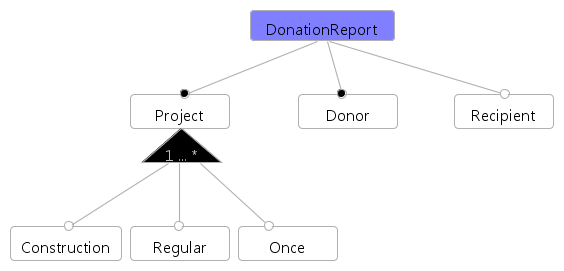
\includegraphics[scale=0.65]{featureDiagram.png}
	\caption{Feature Diagram of Donation Report}
	\label{feature diagram}
\end{figure}

Furthermore, a class diagram of the donation report system is also made to see the relationship between the class and the attributes needed of each class. 

\begin{figure}
	\centering
	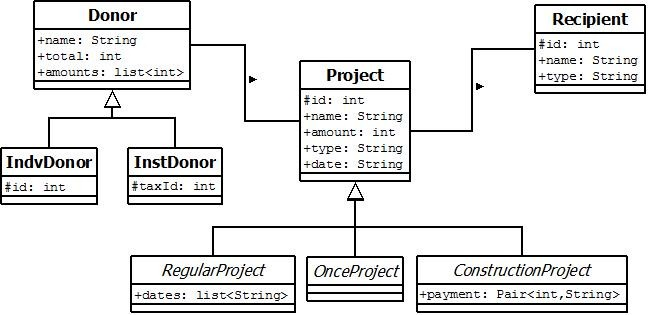
\includegraphics[scale=0.65]{classDiagram.jpg}
	\caption{Class Diagram of Donation Report}
	\label{class diagram}
\end{figure}

The introduction part of this paper describes the background problem, motivation, and requirement analysis of the case study. The next section of this paper discusses the mapping technique from delta oriented programming into relational database introduced by this research. This section discusses about relational database schema elements, core ABS and delta modules, and introduces mismatch between ABS language and relational database schema. The following section describes the implementation of the case study and implementation of mapping technique on the case study. This section discusses the expected results, case study implementation in ABS, implementation of mapping technique on the case study, and evaluation. The last section provides the conclusion and the future work of this research.

\section{Mapping Technique}
This section describes the proposal of mapping technique used in the mapping process from ABS code into relational database schema. The mapping technique is defined based on relational database schema and the basic syntax of ABS modules. This section will be divided into several parts as follows:
\begin{enumerate}
	\item The steps used in defining the mapping technique
	\item The elements of relational database schema as the target of the mapping
	\item The mapping of core ABS component and delta module into relational database schema elements
	\item The mismatch between ABS language and relational database schema and the solution for it
\end{enumerate}

\subsection{The Methodology of Mapping Technique}
ORM(Object Relational Mapping) does the mapping works between object model in object oriented programming and relational model in relational database. There are three type of perspective used by ORM to do the mapping, those are:
\begin{enumerate}
	\item Metadata-oriented, which uses metadata as the input to generate the mapping code
	\item Application-oriented, which starts from object-oriented application to do the mapping
	\item Database-oriented, which does the mapping from the database.
\end{enumerate}

The mapping technique proposed in this research uses the last perscpective used by ORM, which is database-oriented approach. Hence the approach to do the mapping is started from the target of the mapping, which is the relational database schema. The following are the steps used in defining the mapping technique:

\begin{enumerate}
	\item Analyze the aspect of relational database schema\\
	In this step we obtain the elements of relational database schema and what is needed to create a relational database schema. Based on those elements, we define the information which needs to be provided by the ABS model so it can be generated into database schema.
	\item Analyze the component of ABS modules\\
	In this step we analyze the component of ABS modules and their syntax. Then we define the components which provide the information needed to create a relational database schema. After that, those components are mapped into the corresponding relational database schema’s elements.
	\item Analyze the mismatch between ABS language and relational database schema and define the solutions\\
	This step is done by revisiting step 1 and step 2. In this step we find the elements of relational database schema which are not provided by the ABS language. Furthermore, we also find the components of ABS modules which are not available in relational database concept. So we define the solution to the mismatch, by considering the constraints of each concept.
\end{enumerate}

\subsection{Relational Database Schema Elements}
The main elements of relational database schema are tables and constraints. Below are the components of a relational database schema.

\begin{table}[]
	\centering
	\caption{ The Representation of Relational Database Schema Components}
	\label{my-label}
	\begin{tabular}{|l|l|l|l|}
		\hline
		\multirow{9}{*}{schema} & \multirow{7}{*}{table} & \multirow{3}{*}{attribute}   & name              \\ \cline{4-4} 
		&                        &                              & data type         \\ \cline{4-4} 
		&                        &                              & {[}constraints{]} \\ \cline{3-4} 
		&                        & \multicolumn{2}{c|}{\multirow{2}{*}{:}}          \\
		&                        & \multicolumn{2}{c|}{}                            \\ \cline{3-4} 
		&                        & \multirow{2}{*}{constraints} & Primary Key       \\ \cline{4-4} 
		&                        &                              & {[}Foreign Key{]} \\ \cline{2-4} 
		& \multicolumn{3}{c|}{\multirow{2}{*}{:}}                                   \\
		& \multicolumn{3}{c|}{}                                                     \\ \hline
	\end{tabular}
\end{table}

In a database schema there will be at least one table. In each table, there will be at least one attribute, there must be one primary key, and there could be any number of foreign keys. In each attribute, there must be an attribute name, there must be an attribute data type, and there could be any attribute constraints. Hence, we should extract the ABS code to get the information about:

\begin{itemize}
	\item table(s)
	\begin{itemize}	
		\item attribute(s)
			\begin{itemize}
				\item attribute name
				\item attribute data type
				\item attribute constraint(s)
			\end{itemize}
		\item primary key
		\item foreign key
	\end{itemize}
\end{itemize}

\subsection{Core ABS and Delta Modules}
Based on the analysis on previous section, the information needed to generate a database schema is provided by the core modules of ABS. However ABS implements delta-oriented programming. Hence, we should also consider the modification done by the delta modules which will affect the ABS core. 	

\subsubsection*{Core ABS Mapping}

Core ABS contains at least one module. In each module, there could be any import and export from other modules, any interface declarations, any class declarations, any data type declarations, any function declarations, and main block. For every declared interface, there could be any abstract method declarations. For every class, there could be any class parameters, any interfaces implemented, any fields, and any methods. For every class parameter, there must be a data type and a name. Whereas for every field in a class, there must be a data type and a name, and there could be an initial value. 

% Please add the following required packages to your document preamble:
% \usepackage{multirow}
\begin{table}[]
	\centering
	\caption{The Representation of Core ABS Components}
	\label{my-label}
	\begin{tabular}{|l|l|l|l|l|}
		\hline
		\multirow{23}{*}{core} & \multirow{22}{*}{module} & \multicolumn{3}{l|}{export}                                             \\ \cline{3-5} 
		&                          & \multicolumn{3}{l|}{import}                                             \\ \cline{3-5} 
		&                          & \multirow{2}{*}{interface} & \multicolumn{2}{l|}{abstract method}       \\ \cline{4-5} 
		&                          &                            & \multicolumn{2}{c|}{:}                     \\ \cline{3-5} 
		&                          & \multicolumn{3}{c|}{:}                                                  \\ \cline{3-5} 
		&                          & \multirow{11}{*}{class*}   & \multirow{2}{*}{parameter*}  & data type*  \\ \cline{5-5} 
		&                          &                            &                              & name*       \\ \cline{4-5} 
		&                          &                            & \multicolumn{2}{c|}{:}                     \\ \cline{4-5} 
		&                          &                            & \multicolumn{2}{l|}{implemented interface} \\ \cline{4-5} 
		&                          &                            & \multicolumn{2}{c|}{:}                     \\ \cline{4-5} 
		&                          &                            & \multirow{3}{*}{field*}      & data type*  \\ \cline{5-5} 
		&                          &                            &                              & name*       \\ \cline{5-5} 
		&                          &                            &                              & value*      \\ \cline{4-5} 
		&                          &                            & \multicolumn{2}{c|}{:}                     \\ \cline{4-5} 
		&                          &                            & \multicolumn{2}{l|}{method}                \\ \cline{4-5} 
		&                          &                            & \multicolumn{2}{c|}{:}                     \\ \cline{3-5} 
		&                          & \multicolumn{3}{c|}{:}                                                  \\ \cline{3-5} 
		&                          & \multicolumn{3}{l|}{data type declaration}                              \\ \cline{3-5} 
		&                          & \multicolumn{3}{c|}{:}                                                  \\ \cline{3-5} 
		&                          & \multicolumn{3}{l|}{function declaration}                               \\ \cline{3-5} 
		&                          & \multicolumn{3}{c|}{:}                                                  \\ \cline{3-5} 
		&                          & \multicolumn{3}{l|}{main block}                                         \\ \cline{2-5} 
		& \multicolumn{4}{c|}{:}                                                                             \\ \hline
	\end{tabular}
\end{table}

In Table 6, the components that are related with the information needed to generate a database schema are marked with (*). Note that any imported and exported items will not affect the database schema. Furthermore, any methods in the interface and class, and also functional declaration will not affect the database schema. However, the interface and data type declaration are related with the database schema, because the implemented interface affect the type of the object and data type declared could be the data type of a class parameter or a field. These issues will be discussed in the next section. Table 7 contains the mapping of each component of a module with relational database schema components.

\begin{table}[]
	\centering
	\caption{Mapping of ABS Module Component into Database Schema Component}
	\label{my-label}
	\begin{tabular}{|l|l|l|}
		\hline
		\multicolumn{1}{|c|}{\cellcolor[HTML]{C0C0C0}}                                                   & \multicolumn{1}{c|}{\cellcolor[HTML]{C0C0C0}}                                                                               & \multicolumn{1}{c|}{\cellcolor[HTML]{C0C0C0}}                                                                                                      \\
		\multicolumn{1}{|c|}{\multirow{-2}{*}{\cellcolor[HTML]{C0C0C0}\textbf{Module Component}}}        & \multicolumn{1}{c|}{\multirow{-2}{*}{\cellcolor[HTML]{C0C0C0}\textbf{}}}                                                    & \multicolumn{1}{c|}{\multirow{-2}{*}{\cellcolor[HTML]{C0C0C0}\textbf{Database Schema Component}}}                                                  \\ \hline
		Class                                                                                            & --\textgreater                                                                                                              & Table                                                                                                                                              \\ \hline
		&                                                                                                                             &                                                                                                                                                    \\
		&                                                                                                                             &                                                                                                                                                    \\
		&                                                                                                                             &                                                                                                                                                    \\
		\multirow{-4}{*}{\begin{tabular}[c]{@{}l@{}}Class Parameter\\ - Data type\\ - Name\end{tabular}} & \multirow{-4}{*}{\begin{tabular}[c]{@{}l@{}}--\textgreater\\ --\textgreater\\ --\textgreater\\ --\textgreater\end{tabular}} & \multirow{-4}{*}{\begin{tabular}[c]{@{}l@{}}Attribute\\ - Attribute type\\ - Attribute name\\ - NOT NULL constraint\end{tabular}}                  \\ \hline
		&                                                                                                                             &                                                                                                                                                    \\
		&                                                                                                                             &                                                                                                                                                    \\
		&                                                                                                                             &                                                                                                                                                    \\
		\multirow{-4}{*}{\begin{tabular}[c]{@{}l@{}}Field\\ - Data type\\ - Name\\ -Value\end{tabular}}  & \multirow{-4}{*}{\begin{tabular}[c]{@{}l@{}}--\textgreater\\ --\textgreater\\ --\textgreater\\ --\textgreater\end{tabular}} & \multirow{-4}{*}{\begin{tabular}[c]{@{}l@{}}Attribute\\ - Attribute type\\ - Attribute name\\ - Default value for DEFAULT constraint\end{tabular}} \\ \hline
	\end{tabular}
\end{table}

A class in ABS is considered as a relation or table in relational database schema. Furthermore, the class parameters and the fields of a class will be considered as the attributes or columns in relational database schema, with the data type as the attribute type and the name as the attribute name. Class parameters in ABS must be initialized when creating a new object. Hence, attributes generated from class parameter will have NOT NULL constraints. In ABS, a field declaration in a class declaration must be initialized with a certain value. Hence the value will be used as the default value in the database schema. In other words, objects in ABS will be considered as tuples or rows in the relational database schema.

\subsubsection*{Delta Modules}
Table 8 contains the analysis between the possible modifications done by delta modules and the effects on the database schema. Note that every modification related to method and function will not affect the database schema.

\begin{table}[]
	\centering
	\caption{Analysis of Delta Module Modification Effect on Database Schema}
	\label{my-label}
	\begin{tabular}{|l|l|l|}
		\hline
		\multicolumn{1}{|c|}{\cellcolor[HTML]{C0C0C0}}                                                                                                      & \multicolumn{1}{c|}{\cellcolor[HTML]{C0C0C0}}                                            & \multicolumn{1}{c|}{\cellcolor[HTML]{C0C0C0}}                                                     \\
		\multicolumn{1}{|c|}{\multirow{-2}{*}{\cellcolor[HTML]{C0C0C0}\textbf{Possible Modification by Delta}}}                                             & \multicolumn{1}{c|}{\multirow{-2}{*}{\cellcolor[HTML]{C0C0C0}\textbf{}}}                 & \multicolumn{1}{c|}{\multirow{-2}{*}{\cellcolor[HTML]{C0C0C0}\textbf{Effect to Database Schema}}} \\ \hline
		Adding new class                                                                                                                                    & --\textgreater                                                                           & Add table                                                                                         \\ \hline
		Adding new interface                                                                                                                                & --\textgreater                                                                           & -                                                                                                 \\ \hline
		\begin{tabular}[c]{@{}l@{}}Modifying class\\ - Add attribute\\ - Remove attribute\\ - Add/remove method\end{tabular}                                & \begin{tabular}[c]{@{}l@{}}--\textgreater\\ --\textgreater\\ --\textgreater\end{tabular} & \begin{tabular}[c]{@{}l@{}}Add column\\ Remove column\\ -\end{tabular}                            \\ \hline
		\begin{tabular}[c]{@{}l@{}}Modify interfaces\\ (modify abstract methods)\end{tabular}                                                               & --\textgreater                                                                           & -                                                                                                 \\ \hline
		Remove class                                                                                                                                        & --\textgreater                                                                           & Remove table                                                                                      \\ \hline
		\begin{tabular}[c]{@{}l@{}}Modify functional entities\\ - Add and modify data types\\ - Add and modify type synonyms\\ - Add functions\end{tabular} & \begin{tabular}[c]{@{}l@{}}--\textgreater\\ --\textgreater\\ --\textgreater\end{tabular} & \begin{tabular}[c]{@{}l@{}}-\\ -\\ -\end{tabular}                                                 \\ \hline
	\end{tabular}
\end{table}



\subsection{Mismatch between ABS Language and Relational Database Schema}
There are several mismatches between ABS language and relational database schema. These mismatches include primary key in relational database, predefined data type in ABS, parametric data type in ABS, object type in ABS, and referential integrity in relational database.

\subsubsection{Primary Key in Relational Database}

Primary key is used as the identity of the tuple in the relation. It is important especially in accessing the tuple and when the tuple has relationship with another tuple in another relation. Basically, primary key can be considered as the object identity in object-oriented concepts. However, in ABS, there is no concept of primary key as in relational database. Hence, we will use annotations in ABS to provide the information about primary key in class declarations in ABS.

ABS supports annotations to enrich an ABS model with additional information. Annotations in ABS can appear before any declaration and type usage in ABS programs. In this case, we will use annotation [PK] to describe a class parameter or a field of a class as the primary key of the relation. Note that a relation can have one or more attributes as the primary key. Hence, in a class declaration in ABS the annotation [PK] can be used more than once, either in class parameter or in field declaration. Figure 3 is an example of using annotation in declaring the primary key in class declaration in ABS.

\begin{figure}
	\centering
	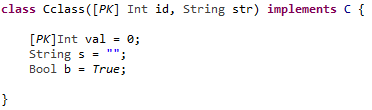
\includegraphics[scale=0.7]{41.png}
	\caption{Primary Key Declaration using Annotations in ABS}
	\label{primary key}
\end{figure}

\subsubsection{Predefined Data Type in ABS}
There are several differences in data types between ABS and SQL. Table 9 contains the mapping of data types in ABS to basic data types in SQL.

\begin{table}[]
	\centering
	\caption{The Mapping of Predefined Data Types in ABS to Basic Data Types in SQL}
	\label{my-label}
	\begin{tabular}{|l|l|l|}
		\hline
		\multicolumn{1}{|c|}{\cellcolor[HTML]{C0C0C0}}                                                                                               & \multicolumn{1}{c|}{\cellcolor[HTML]{C0C0C0}}                            & \multicolumn{1}{c|}{\cellcolor[HTML]{C0C0C0}}                                                                                         \\
		\multicolumn{1}{|c|}{\multirow{-2}{*}{\cellcolor[HTML]{C0C0C0}\textbf{\begin{tabular}[c]{@{}c@{}}ABS \\ Predefined Data Type\end{tabular}}}} & \multicolumn{1}{c|}{\multirow{-2}{*}{\cellcolor[HTML]{C0C0C0}\textbf{}}} & \multicolumn{1}{c|}{\multirow{-2}{*}{\cellcolor[HTML]{C0C0C0}\textbf{\begin{tabular}[c]{@{}c@{}}SQL\\ Basic Data Type\end{tabular}}}} \\ \hline
		Bool                                                                                                                                         & --\textgreater                                                           & Boolean                                                                                                                               \\ \hline
		Unit                                                                                                                                         & --\textgreater                                                           & NULL                                                                                                                                  \\ \hline
		Int                                                                                                                                          & --\textgreater                                                           & INT                                                                                                                                   \\ \hline
		Rat                                                                                                                                          & --\textgreater                                                           & FLOAT                                                                                                                                 \\ \hline
		String                                                                                                                                       & --\textgreater                                                           & VARCHAR(n)                                                                                                                            \\ \hline
		Fut\textless T\textgreater*                                                                                                                   &                                                                          &                                                                                                                                       \\ \hline
		List\textless A\textgreater**                                                                                                                 &                                                                          &                                                                                                                                       \\ \hline
	\end{tabular}
\end{table}

Fut\textless T\textgreater is a data type that represents a future, as a result of an asynchronous method call. In this research data type Fut\textless T\textgreater is not mapped into any SQL basic data types. Data type List\textless A\textgreater is one of the parametric data types in ABS. Hence the mapping of it will be discussed in the next section.

Regarding the data type, ABS also has abstract data type declarations. For abstract data type, only the functions that operate on them are known to the client, but not its data type constructors. Hence the initialization or modification of fields which have this type is usually done by calling the functions. This can be realized in ABS by putting such a data type in its own module and by only exporting the data type and its functions, without exporting the constructors. However, abstract data types could also appear in the class declaration, either as the data type of the class parameter or as the data type of the field. This is handled by assigning the name of the abstract data type as the attribute name, whereas the attribute type is assigned as VARCHAR(n).

Another thing to be noted is the maximum length of the VARCHAR type. For this research, the length of the string is capped at 30 characters. Hence every String data type in ABS will be mapped to VARCHAR(30) in SQL database schema.

Besides the predefined data types mentioned above, there are also several predefined data types in ABS Standard Library which can break one of the constraints of the relational database. Those data types are Pair and Triple. Below is the data type declaration of Pair and Triple in ABS Standard Library.

\begin{figure}
	\centering
	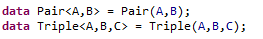
\includegraphics[scale=0.7]{PAIR.png}
	\label{primary key}
\end{figure}

A field or class parameter with Pair or Triple type will have more than one value. Hence, these data types will result multivalued attributes, which break the domain constraints. To avoid this, the value of Pair data type and Triple data type will be separated into several attributes in database schema. For Pair data type, there will be two attributes. The first attribute will have [fieldName]0 as the attribute name, and the attribute type of it will be the first type parameter defined inside the angle brackets (\textless \textgreater). Whereas the second attribute will have [fieldName]1 as the attribute name, and the attribute type of it will be the second type parameter defined inside the angle brackets (\textless \textgreater).

As for the Triple data type, there will be three attributes. The first attribute will have [fieldName]0 as the attribute name, and the attribute type of it will be the first type parameter defined inside the angle brackets (\textless \textgreater). Whereas the second attribute will have [fieldName]1 as the attribute name, and the attribute type of it will be the second type parameter defined inside the angle brackets (\textless \textgreater). And the third attribute will have [fieldName]2 as the attribute name, and the attribute type of it will be the third type parameter defined inside the angle brackets (\textless \textgreater). 

\subsubsection{Parametric Data Type in ABS}
In ABS, parametric data types usually used to define general-purpose data types, such as lists, sets, and maps. Those three are already defined in the ABS Standard Library. However, these parametric data types are breaking the domain constraints of the relational database schema, because parametric data types will produce multivalued attribute. As the solution, multivalued attributes must be represented by separate relations. Hence, every class parameter or field in ABS with list, set, or map type, will be generated as a new table in database schema.

For a field or class parameter with list type, the name of the new table will be List[className]. Then the name of the field will be the attribute name in the new table. The attribute type of this new attribute is the type parameter defined inside angle brackets (\textless \textgreater). Besides that this new table will have the primary key attributes of the class as the additional attributes. The name of the additional attribute will be [attributeName]\_[className]. The primary key of this new table is the whole attributes of it. This new table will have at least one foreign key, which is every additional attribute will refer to the corresponding attribute of the class. 

For a field or class parameter with set type, the name of the new table will be Set[className]. Then the name of the field will be the attribute name in the new table. The attribute type of this new attribute is the type parameter defined inside angle brackets (\textless \textgreater). Besides that this new table will have the primary key attributes of the class as the additional attributes. The name of the additional attribute will be [attributeName]\_[className]. The primary key of this new table is the whole attributes of it. This new table will have at least one foreign key, which is every additional attribute will refer to the corresponding attribute of the class.

For a field or class parameter with map type, the name of the new table will be Map[className]. Because one element in a map contains two things, those are key and value, this new table will have two attributes. The first attribute will contain the key, and the attribute name will be [fieldName]0. The attribute type of the first attribute will be the first type parameter defined inside angle brackets (\textless \textgreater). The second attribute will contain the value, and the attribute name will be [fieldName]1. The attribute type of the second attribute will be the second type parameter defined inside angle brackets (\textless \textgreater). Besides that this new table will have the primary key attributes of the class as the additional attributes. The name of the additional attribute will be [attributeName]\_[className]. The primary key of this new table is the whole attributes of it. This new table will have at least one foreign key, which is every additional attribute will refer to the corresponding attribute of the class.

\subsubsection{Object type in ABS}
Only interfaces can be used as types in ABS. Hence the type of the object is based on the interfaces implemented by the class. Since class can implement an arbitrary number of interfaces and an interface can extend arbitrary number of other interfaces, there will be many possible types for the object of a class. Moreover we could not define the object type in the class declaration, because this information will only be available at runtime.

To provide the information of the object type, we will create an additional table for each interface implemented in core ABS. The additional table for an interface will have several attributes. The first attribute is the generated id. The rest of the attributes are all primary key attributes of all classes which implement the interface. Note that the implemented interfaces are not only the interfaces declared in class declarations, but also include the interfaces extended by those interfaces. In other words, the information of interface hierarchy is needed to define all the classes which implement a certain interface. The primary key attributes of each class in the additional table will refer to the primary key attributes of the table of the class as the primary key. And the primary key of the additional table will be the attribute which contains the generated id. Later, when a new object is created, a unique id is generated. Then the unique id along with the primary key value of the object will be stored in the interface type table.

\begin{figure}
	\centering
	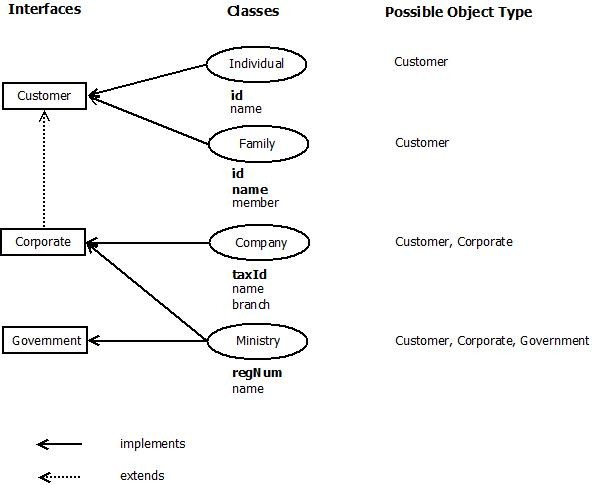
\includegraphics[scale=0.6]{sample.jpg}
	\caption{The Example of Retrieving Object Type}
	\label{sample}
\end{figure}

Figure 4 is the example to describe the explanation above. There are three interfaces; those are Customer, Corporate, and Government. The Corporate interface extends Customer interface. Then there are four classes; those are Individual, Family, Company, and Ministry. The Individual class implements Customer interface. The Individual class has id and name as the attributes, with id as the primary key. The Family class implements Customer interface. The Family class has id, name, and member as the attributes, with id and name as the primary key. The Company class implements Corporate interface. The Company class has taxId, name, and branch as the attributes, with taxId as the primary key. The Ministry class implements Corporate interface and Government interface. The Ministry class has regNum and name as the attributes, with regNum as the primary key. This situation is represented by Figure 4. 

Based on the interface hierarchy, the possible object type for Individual class and Family class is Customer. The possible object types for Company class are Customer and Corporate, whereas the possible object types for Ministry class are Customer, Corporate, and Government. Hence, the database schema diagram will be as shown in Figure 5.

\begin{figure}
	\centering
	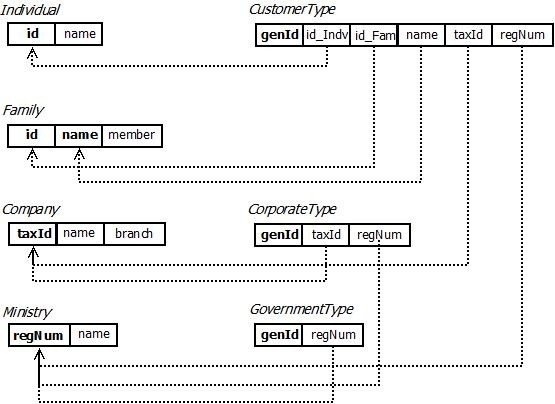
\includegraphics[scale=0.7]{db1.jpg}
	\caption{Database Schema Diagram}
	\label{sample}
\end{figure}

\subsubsection{Referential Integrity in Relational Database}
There is another condition in ABS where the referential integrity constraint in relational database could be violated; that is when a class declaration has other objects as the class parameter or field. ABS, which is object-oriented, enables an object to have another object as its field. When a field is generated as the attribute in relational database, it is impossible to store the whole information of an object in an attribute. Hence, the solution is every time there is a class parameter or field declaration has interface type as the data type, the attribute generated will only contain the generated id of the object which is stored in the interface type table. This attribute will be the foreign key which refers to the primary key of the inference type table.

To describe the explanation above, we will use the same situation as the example beforehand. We add a new interface called Account. This interface is implemented by AccountImpl class, which has id, owner, and balance as the attributes, and the attribute id is the primary key. Note that one of the attribute use interface type as the data type; that is customer. This additional situation is described by Figure 6 below.

\begin{figure}
	\centering
	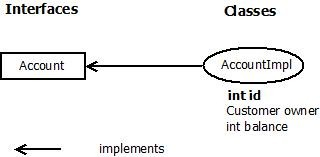
\includegraphics[scale=0.6]{sample2.jpg}
	\caption{Account Interface and AccountImpl Class}
	\label{sample}
\end{figure}

Figure 7 presents the relational database schema based on the explanation above.

\begin{figure}
	\centering
	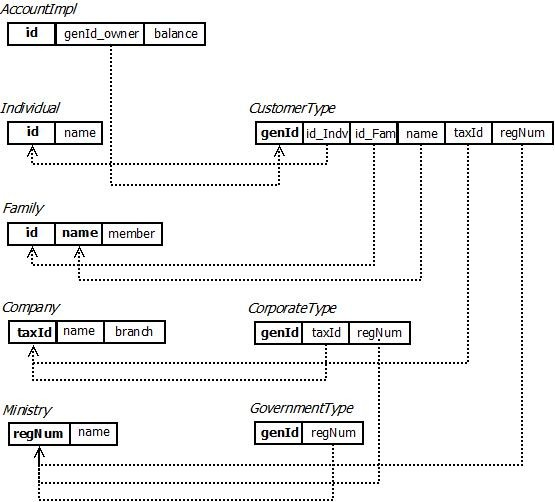
\includegraphics[scale=0.7]{db2.jpg}
	\caption{Database Schema Diagram with AccountImpl Class}
	\label{sample}
\end{figure}


\section{Implementation of Mapping Technique towards Case Study}
This section presents the implementation of the case study and implementation of the mapping technique of the case study. The requirements and the design of the case study were already presented in the Introduction. The presentation of this section starts with the expected results of the mapping technique applied to the case study. The next subsection discusses the implementation of the case study in ABS. The mapping technique is then implemented on the ABS code of the case study to generate the database schema for each product. The last subsection is the evaluation towards the generated database schema based on the expected results defined before.

\subsection{The Expected Results}
Below are the possible products which can be produced in this software product line:
\begin{enumerate}
	\item Once Project: this is the base product, which will store the list of once projects and the donors
	\item Regular Project: this product will store the list of regular projects and the donors.
	\item Construction Project: this product will store list of construction projects
	\item Once Project with Recipient: this product will store list of once projects, donors, and recipients.
	\item Regular Project with Recipient: this product will store list of regular projects, donors, and recipients.
	\item Construction Project with Recipient: this product will store list of construction projects, donors, and recipients.
\end{enumerate}

Note that, from the class diagram there are two types of donors, those are individual donor and institutional donor, whereas the type for project will be  
realized using delta modeling in ABS. Figure 8 contains the schema diagrams for each class in the class diagram.

\begin{figure}
	\centering
	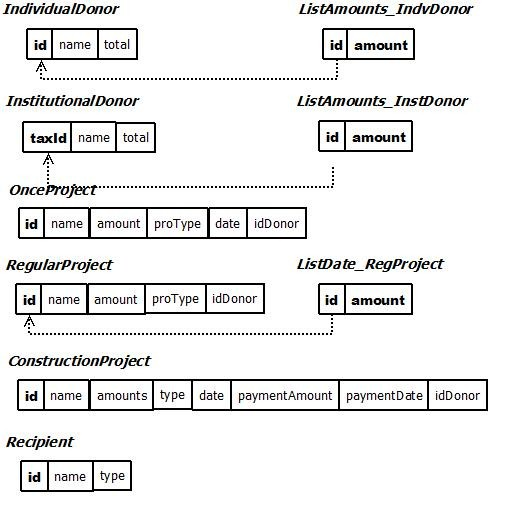
\includegraphics[scale=0.7]{db3.jpg}
	\caption{Expected Schema Diagram for each Class of Case Study}
	\label{Figure 8}
\end{figure}

Now we will define the database schema for each possible product mentioned above. The database schema will be represented by the schema diagram. The first product, Once project, only realizes feature Donor and feature Project. Figure 9 is the expected database schema.

\begin{figure}
	\centering
	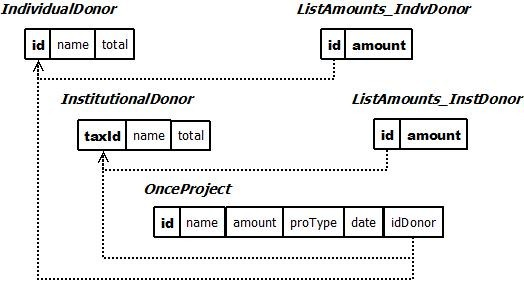
\includegraphics[scale=0.7]{db4.jpg}
	\caption{Expected Schema Diagram for the First Product}
	\label{Figure 9}
\end{figure}

Note that, it is impossible for an attribute to refer two different attributes in the same time. This case is already solved by the mapping technique in ABS, and the result will be presented in the next section. The second product is Regular project, which realizes feature Donor and feature Regular project, with the expected schema diagram shown by Figure 10.

\begin{figure}
	\centering
	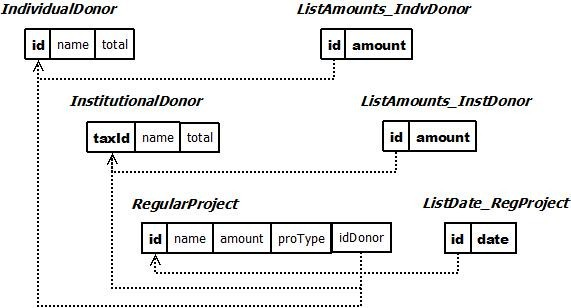
\includegraphics[scale=0.7]{db5.jpg}
	\caption{Expected Schema Diagram for the Second Product}
	\label{Figure 10}
\end{figure}

The third product is Construction project, which realizes feature Donor and feature Construction project, with the expected schema diagram shown by Figure 11.

\begin{figure}
	\centering
	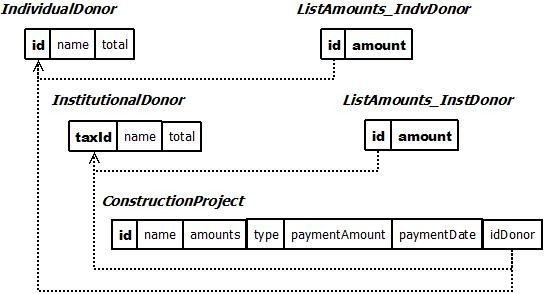
\includegraphics[scale=0.7]{db6.jpg}
	\caption{Expected Schema Diagram for the Third Product}
	\label{Figure 11}
\end{figure}

The fourth product realizes feature Donor, feature Once project, and feature Recipient. There will be a foreign key from relation Project to relation Recipient to represent the association between these relations. The expected schema diagram is represented by Figure 12.

\begin{figure}
	\centering
	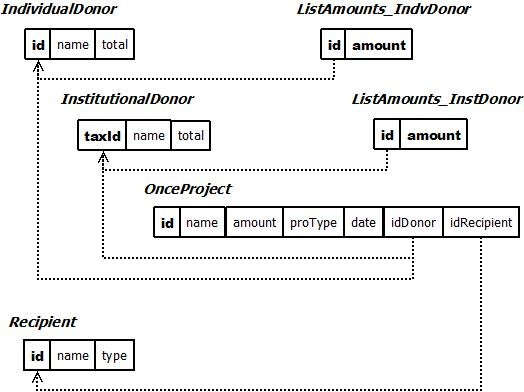
\includegraphics[scale=0.7]{db7.jpg}
	\caption{Expected Schema Diagram for the Fourth Product}
	\label{Figure 12}
\end{figure}

The fifth product realizes feature Donor, feature Regular project, and feature Recipient. There will be a foreign key from relation Project to relation Recipient to represent the association between these relations. The expected schema diagram is represented by Figure 13.

\begin{figure}
	\centering
	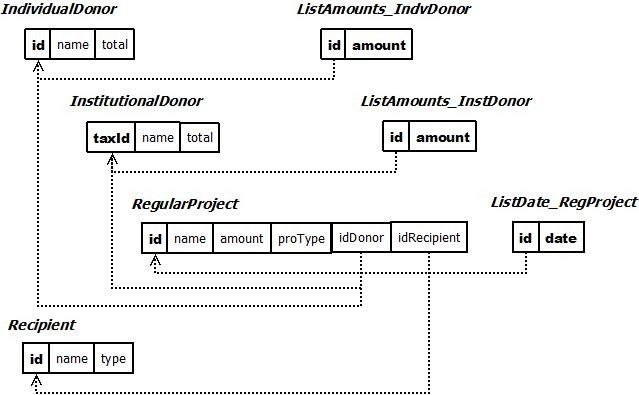
\includegraphics[scale=0.7]{db8.jpg}
	\caption{Expected Schema Diagram for the Fifth Product}
	\label{Figure 13}
\end{figure}

The sixth product realizes feature Donor, feature Construction project, and feature Recipient. There will be a foreign key from relation Project to relation Recipient to represent the association between these relations. The expected schema diagram is represented by Figure 14.

\begin{figure}
	\centering
	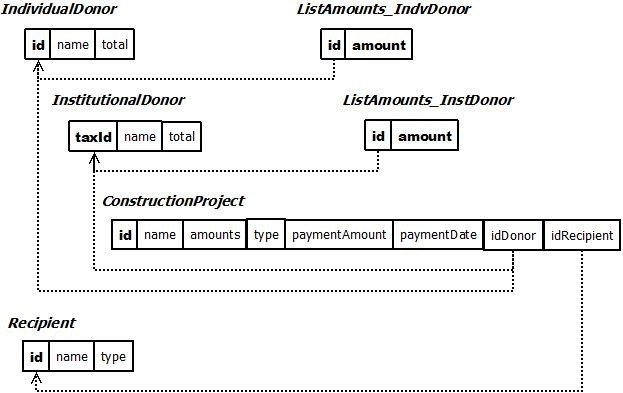
\includegraphics[scale=0.7]{db9.jpg}
	\caption{Expected Schema Diagram for the Sixth Product}
	\label{Figure 14}
\end{figure}

\subsection{Case Study Implementation in ABS}
This section will present the implementation of the case study in ABS.  The case study explained in Section 1 is modeled in ABS with the following modules.

\subsubsection{Module Project}
The first module is module project. This module defines the model of project in ABS. There is an abstract data type declaration which declares the type of the project and constructs its possible value. The abstract data type declaration is followed by function definitions to initialize that abstract data type. This abstract data type is to represent the possible fields of project mentioned in Section 1; those are health, education, empowerment, and disaster relief. And then we define an interface called Project, with several abstract methods. This interface is implemented by the class Project. This class represents the relationship between class donor and class project, by having Donor object as one of its class parameters. Figure 15 shows the ABS code of module Project.

\begin{figure}
	\centering
	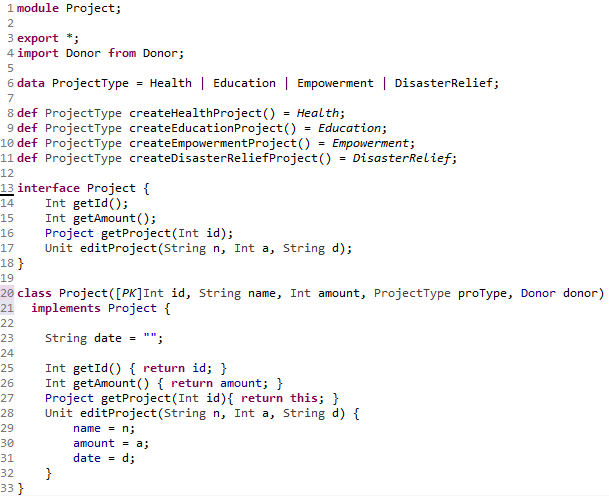
\includegraphics[scale=0.7]{code1.png}
	\caption{The ABS Code of Module Project}
	\label{Figure 15}
\end{figure}

\subsubsection{Module Donor}
This module defines the model of donor in ABS. In this module we declare an interface called Donor, with several abstract methods to represent the behavior of Donor model. This interface is implemented by two classes. The first class is the Individual Donor, and the second class is Institutional Donor. Figure 16 shows the ABS code of module Donor.

\begin{figure}
	\centering
	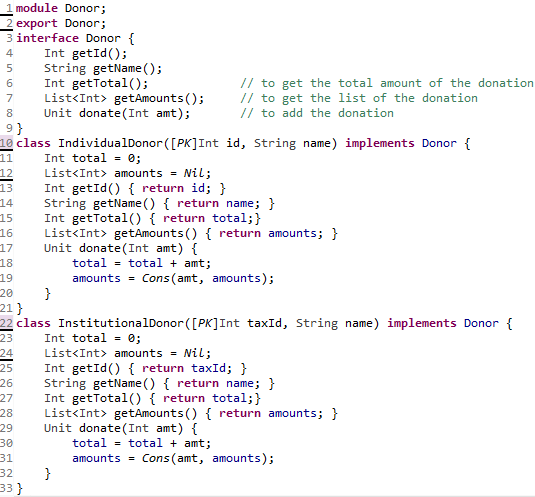
\includegraphics[scale=0.7]{code2.png}
	\caption{The ABS Code of Module Donor}
	\label{Figure 16}
\end{figure}

\subsubsection{Delta Modules}
The delta modules consist of DRegular, DConstuction, and DRecipient. Delta DRegular modifies class Project, removes the field date with String data type, and adds a new date field with parametric data type List\textless String\textgreater. Delta DConstruction modifies class Project, removes the field date with String data type, and add new field called payment which has Pair\textless Int,String\textgreater as the data type. Delta DRecipient adds new abstract data type in module Project, and defines the functions to initialize it. This abstract data type is to represent the type of the recipient, which are individual, institutional, and regional. This delta also adds new interface called Recipient and new class Recipient which implements Recipient interface. To represent the relationship between class Project and class Recipient, delta DRecipient modifies class Project by adding Recipient as new field. The ABS codes of delta modules are shown by Figure 17, Figure 18, and Figure 19.

\begin{figure}
	\centering
	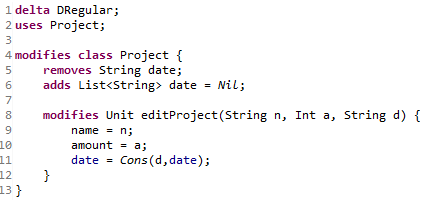
\includegraphics[scale=0.7]{code3.png}
	\caption{The ABS Code of Delta DRegular}
	\label{Figure 17}
\end{figure}

\begin{figure}
	\centering
	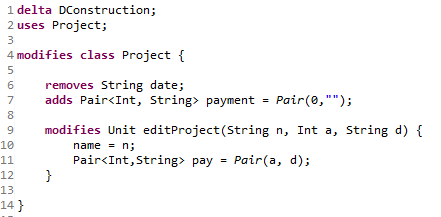
\includegraphics[scale=0.7]{code4.png}
	\caption{The ABS Code of Delta DConstruction}
	\label{Figure 18}
\end{figure}

\begin{figure}
	\centering
	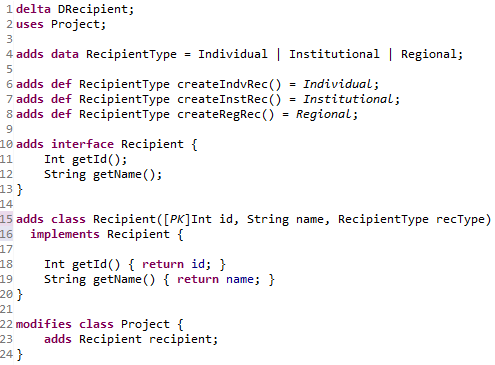
\includegraphics[scale=0.7]{code5.png}
	\caption{The ABS Code of Delta DRecipient}
	\label{Figure 19}
\end{figure}

\subsubsection{Feature Model}
Figure 20 is the feature model in \textmu TVL which represents the feature diagram shown in Figure 1.

\begin{figure}
	\centering
	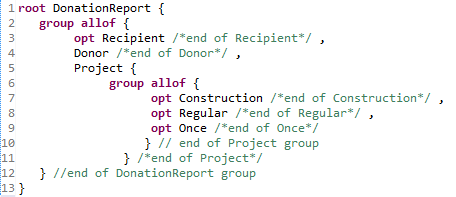
\includegraphics[scale=0.7]{code6.png}
	\caption{The Code of Feature Model of The Case Study}
	\label{Figure 20}
\end{figure}

\subsubsection{Product Line Configuration}
The product line in Figure 21 defines features and the corresponding delta to realize the features. Delta DRegular will be implemented when feature Regular is chosen. Delta DConstruction will be implemented when feature Construction is chosen. And delta DRecipient will be implemented if feature Recipient is chosen.

\begin{figure}
	\centering
	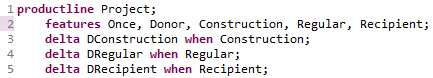
\includegraphics[scale=0.7]{code7.png}
	\caption{The ABS Code of Product Line Configuration}
	\label{Figure 21}
\end{figure}

\subsubsection{Products Declaration}
Figure 22 is the products declaration, as mentioned in the beginning of this section.

\begin{figure}
	\centering
	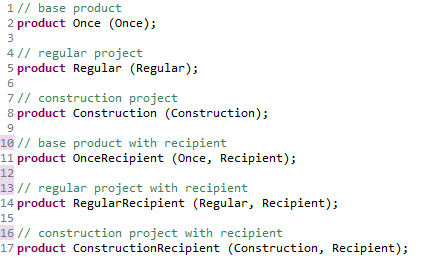
\includegraphics[scale=0.7]{code8.png}
	\caption{The ABS Code of Products Declaration}
	\label{Figure 22}
\end{figure}


\subsection{Implementation of Mapping Technique in the Case Study}
The mapping technique, which is implemented in ABS backend, is implemented in the ABS code of the case study using -dbschema argument in the command line. Below are the results of the mapping technique implementation and the generated database schemas.\\

\emph{generateJava -dbschema -product=Once F:\textbackslash DonationReport\textbackslash *.abs}\\

This command will generate database schema for the first product, as shown in Figure 23.\\

\begin{figure}
	\centering
	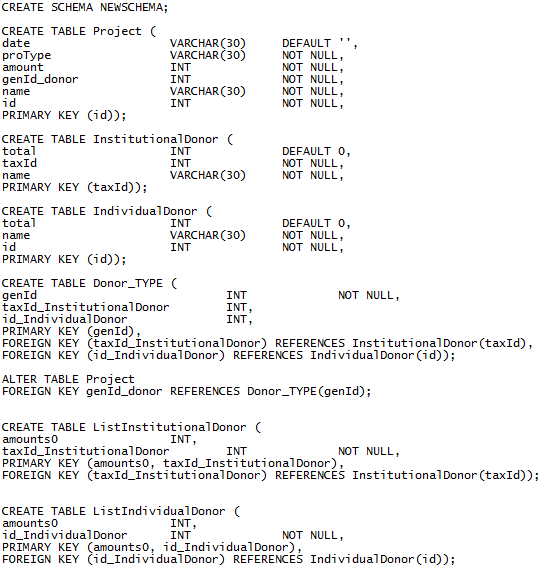
\includegraphics[scale=0.7]{create1.png}
	\caption{The Generated Database Schema of the First Product}
	\label{Figure 23}
\end{figure}

\emph{generateJava -dbschema -product=Regular F:\textbackslash DonationReport\textbackslash *.abs}\\

This command will generate database schema for the second product, as shown in Figure 24.\\

\begin{figure}
	\centering
	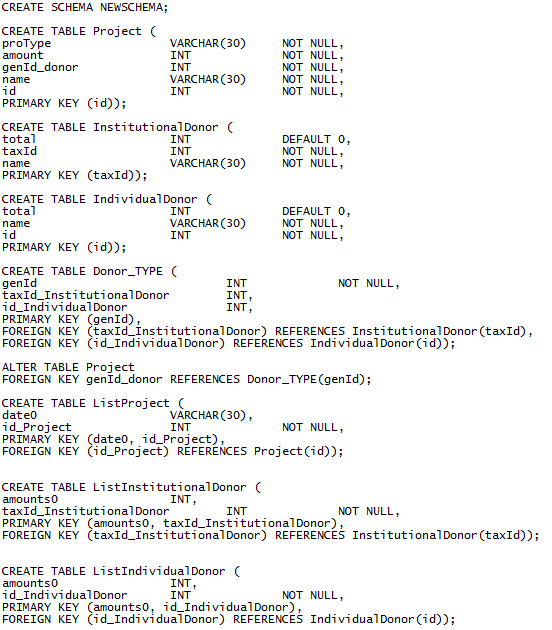
\includegraphics[scale=0.7]{create2.png}
	\caption{The Generated Database Schema of the Second Product}
	\label{Figure 24}
\end{figure}

\emph{generateJava -dbschema -product=Construction F:\textbackslash DonationReport\textbackslash *.abs}\\

This command will generate database schema for the third product, as shown in Figure 25.\\

\begin{figure}
	\centering
	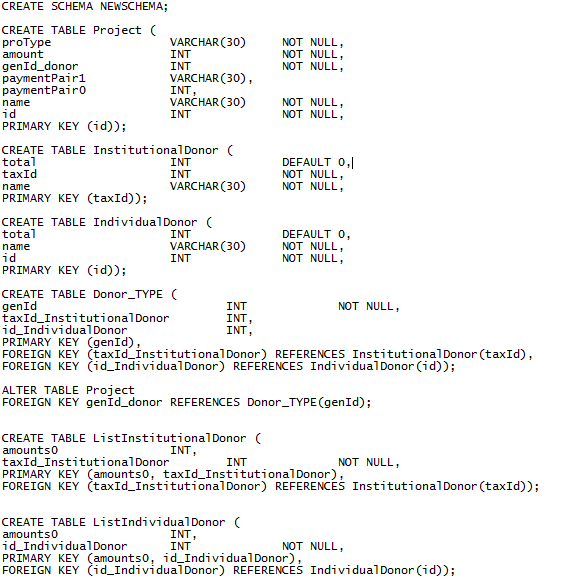
\includegraphics[scale=0.7]{create3.png}
	\caption{The Generated Database Schema of the Third Product}
	\label{Figure 25}
\end{figure}

\emph{generateJava -dbschema -product=OnceRecipient F:\textbackslash DonationReport\textbackslash *.abs}\\

This command will generate database schema for the fourth product, as shown in Figure 26.\\

\begin{figure}
	\centering
	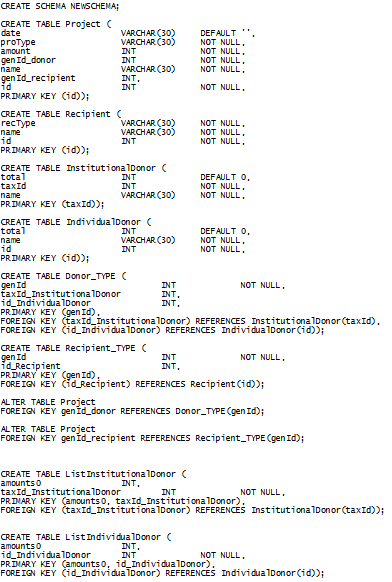
\includegraphics[scale=0.9]{create4.png}
	\caption{The Generated Database Schema of the Fourth Product}
	\label{Figure 26}
\end{figure}

\emph{generateJava -dbschema -product=RegularRecipient F:\textbackslash DonationReport\textbackslash *.abs}\\

This command will generate database schema for the fifth product, as shown in Figure 27.\\

\begin{figure}
	\centering
	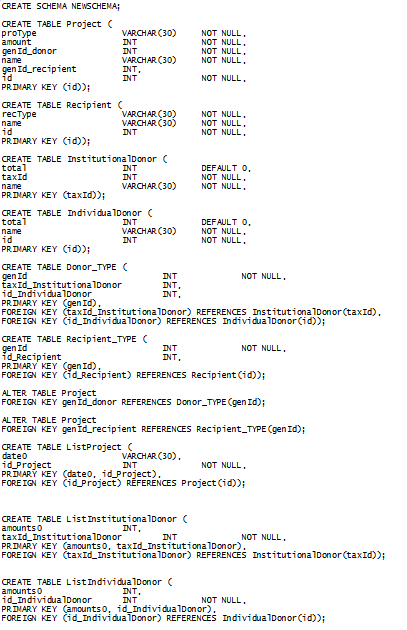
\includegraphics[scale=0.9]{create5.png}
	\caption{The Generated Database Schema of the Fifth Product}
	\label{Figure 27}
\end{figure}

\emph{generateJava -dbschema -product=ConstructionRecipient F:\textbackslash DonationReport\textbackslash *.abs}\\

This command will generate database schema for the sixth product, as shown in Figure 28.\\

\begin{figure}
	\centering
	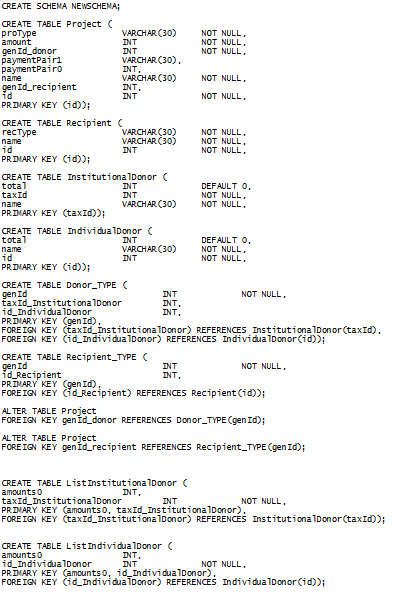
\includegraphics[scale=0.9]{create6.png}
	\caption{The Generated Database Schema of the Sixth Product}
	\label{Figure 28}
\end{figure}


\subsection{Evaluation}
To ease the evaluation process, we will represent the generated database schema as database schema diagrams. The evaluation process is done using hypothetical evaluation, which compares the expected results with the generated results.

Figure 29 is the diagram schema of the generated database schema for the first product.

\begin{figure}
	\centering
	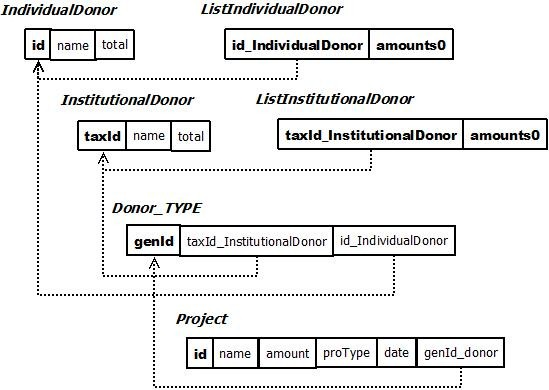
\includegraphics[scale=0.6]{Eval1.jpg}
	\caption{The Diagram Schema of the Generated Database Schema for the First Product}
	\label{Figure 29}
\end{figure}

Figure 30 is the diagram schema of the generated database schema for the second product.

\begin{figure}
	\centering
	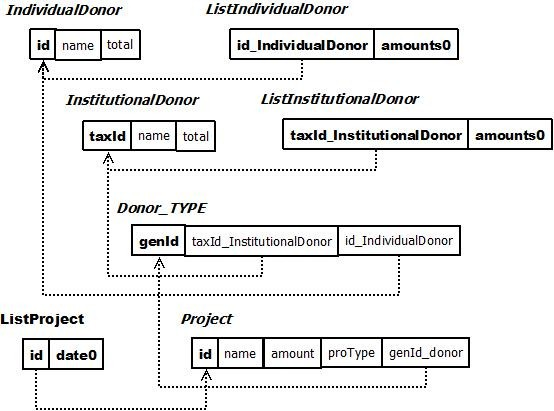
\includegraphics[scale=0.6]{Eval2.jpg}
	\caption{The Diagram Schema of the Generated Database Schema for the Second Product}
	\label{Figure 30}
\end{figure}

Figure 31 is the diagram schema of the generated database schema for the third product.

\begin{figure}
	\centering
	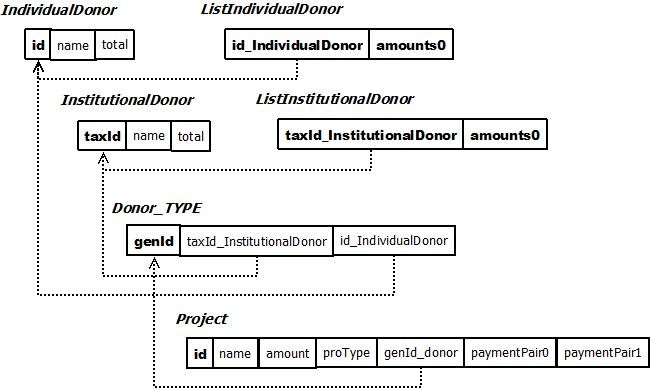
\includegraphics[scale=0.6]{Eval3.jpg}
	\caption{The Diagram Schema of the Generated Database Schema for the Third Product}
	\label{Figure 31}
\end{figure}

Figure 32 is the diagram schema of the generated database schema for the fourth product.

\begin{figure}
	\centering
	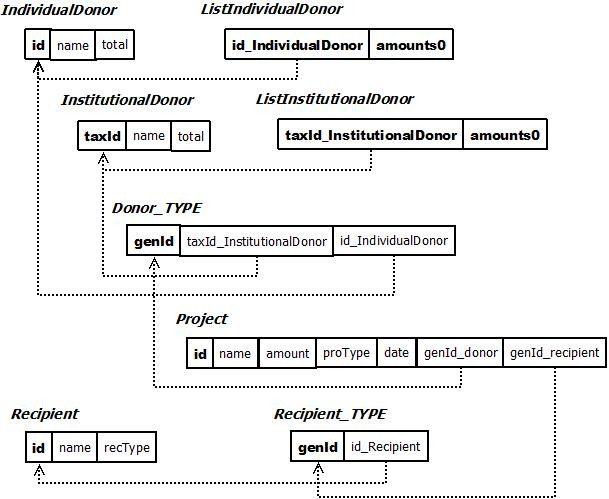
\includegraphics[scale=0.6]{Eval4.jpg}
	\caption{The Diagram Schema of the Generated Database Schema for the Fourth Product}
	\label{Figure 32}
\end{figure}

Figure 33 is the diagram schema of the generated database schema for the fifth product.

\begin{figure}
	\centering
	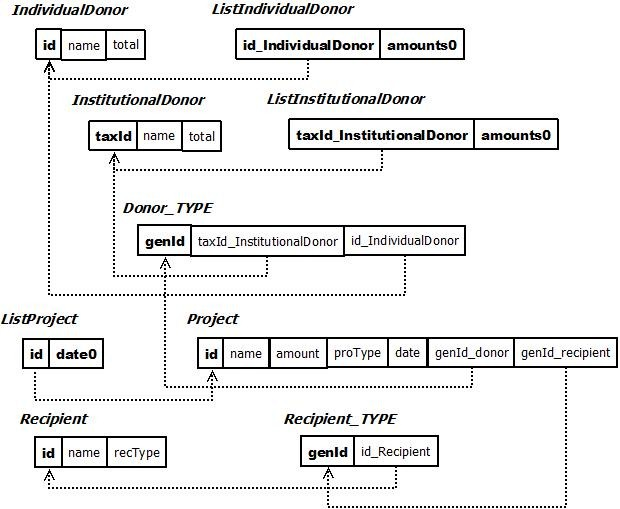
\includegraphics[scale=0.6]{Eval5.jpg}
	\caption{The Diagram Schema of the Generated Database Schema for the Fifth Product}
	\label{Figure 33}
\end{figure}

Figure 34 is the diagram schema of the generated database schema for the sixth product.

\begin{figure}
	\centering
	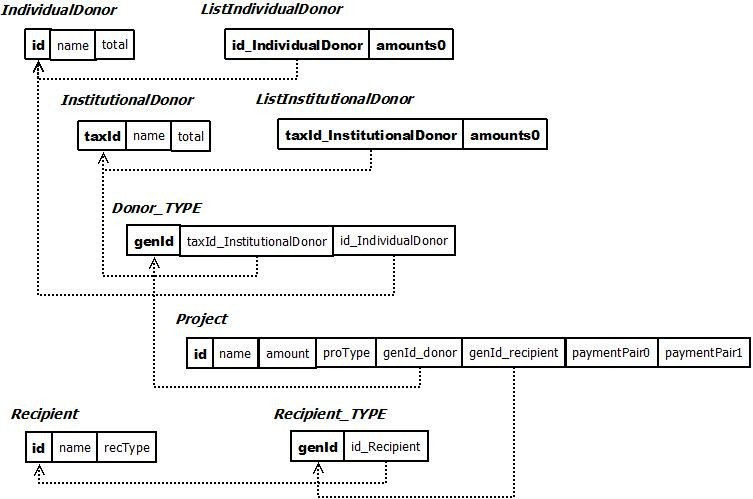
\includegraphics[scale=0.6]{Eval6.jpg}
	\caption{The Diagram Schema of the Generated Database Schema for the Sixth Product}
	\label{Figure 34}
\end{figure}

Based on the comparison between the expected diagram schema and the diagram schema of generated database schema for each product, the results of the mapping are appropriate with the expected results. Furthermore, we can say that the mapping results are even better than the expected results, because the mapping technique is able to solve the issue of more than one reference in one attribute, by implementing intermediate table.

Moreover, the generated database schema is able to fulfill the relational database constraints. The domain constraint is fulfilled by generating a separate relation for multivalued attributes. The key constraint is fulfilled using annotations in ABS, so that every field or class parameter with [PK] annotations will be declared as primary key of the relation. The constraint on NULL is fulfilled by mapping Nil, Unit, EmptySet, and EmptyMap in ABS as NULL. The entity integrity constraints is fulfilled by declaring NOT NULL constraint for primary key attributes and attributes derived from class parameter. The referential integrity constraint is fulfilled by declaring foreign key, when two classes are related by association. 

Besides that, the mapping technique is also able to solve the mismatch between ABS language and relational database concepts, especially the object type issue in ABS. This issue is solved by the mapping technique by generating intermediate table based on the interface type declared in ABS core modules.

By using this mapping technique, we can generate relational database schema directly from ABS model. Hence, it can ease the process of software development, especially software with databases. Moreover, delta-oriented programming implemented by ABS makes product realization in SPLE easier. In other words, this mapping technique can ease the process of product realization in SPLE for software with databases.
 
The case study used in this research is the simplification of real-life case faced by charity organizations. In reality, there are many variations of programs and activities of charity organizations. For this case study, this mapping technique is able to generate any relational database schemas corresponding to each product defined. Each product of this case study represents the variation of charity organizations’ programs.

This mapping technique can be used to map ABS model into relational database schema with following limitations:
 
\begin{enumerate}
	\item Class declaration in ABS model does not have Fut\textless T\textgreater as class parameter data type and/or field data type.
	\item Class declaration on ABS model does not have any class parameter and/or field which has more than one parametric data type as a data type.
	For example: List\textless Pair\textless Int,String\textgreater \textgreater
\end{enumerate}

Any fields or class parameters that have data type as mentioned above will not be mapped into any attribute (column) in relational database schema generated by this mapping technique.


\section{Conclusion and Future Work}
This Section concludes the work and discusses about the future work.

\subsection{Conclusion}
Based on the goal of this research and the evaluation of case study in the previous section, we can conclude:

\begin{enumerate}
	\item Based on the results of this research, delta modeling in ABS can influence the elements of relational database schema.  The elements of relational database schema can be obtained from the core ABS, especially in the class declaration and interface declaration in every module. This base database schema, which is generated from the core ABS, can be affected by the implementation of delta modules. This case happens if the modification by the delta modules related to the class and the fields in a class.
	\item The mapping between ABS modeling and relational database schema is possible to be formulated, by considering the elements and the constraints owned by both sides. The elements which have similarities for both sides can be mapped directly. For example, an attribute of a class is mapped into attribute of a relation. However, there are several mismatches between both sides because of the conceptual differences. This can be solved by implementing some technique so that both sides’ constraints can be fulfilled. Using ABS annotations to declare primary key and generating intermediate table for object type are the solutions to the mismatches.
	\item The mapping technique and product configuration in ABS can be integrated by implementing the mapping technique in ABS backend compiler. The usage of ANTLR and JastAdd by ABS compiler makes the mapping technique integration possible. The mapping technique is implemented in an aspect file, which will later be processed by JastAdd. The aspect file is used to modify the AST classes, which are generated by the JastAdd system from the AST constructed by ANTLR. Moreover, ABS compiler provides ‘-product=’ argument which can be used to generate flattened core ABS by the application of delta modules. By adding ‘-dbschema’ argument to the main program of ABS compiler, we can generate relational database schema from the flattened core ABS by delta modeling implementation, using command line.
	\item The simulation of mapping technique and database schema generation is done using donation report case study. The case study is built based on the simplification of real-life cases faced by charity organizations. Moreover, the case study contains the mismatch issues mentioned before, such as multivalued attributes, object type, and referential integrity. Hence, we can  say that the result of the case study represents the effectiveness of the mapping technique. The evaluation of the case study implementation in the previous section shows that the result of the database schema generation is better than the expected result defined beforehand. Hence, it is safe to say that the mapping technique is effective to generate simple relational database schema from ABS model.
\end{enumerate}

\subsection{Future Work}
Basically this research is the first step of a bigger research that connects ABS to databases. Below is possible future work, which can be done to continue the process of connecting ABS to database.

\begin{enumerate}
	\item The normalization of the generated database schema to fulfill the normal forms in relational database schema.
	\item The implementation of the database operations: retrieval, deletion, and update. These operations will correspond to the method invocation in the main block of ABS. Moreover, this implementation relates to the ABS runtime.
	\item The usage of DBMS for database implementation in ABS: if DBMS will be used in database implementation by ABS, then the connection between ABS and DBMS must be formulated. An application program, in this case is ABS, accesses the database by sending queries or request for data in the DBMS. A query typically causes some data to be retrieved. A transaction done in application program may cause some data to be updated and written in the database. This connection will make ABS as a running application program which is able to access the database through the DBMS.
	\item Maintaining the evolvement of database connected to ABS because of the application requirement changes: requirement changes of application could lead to schema evolution where changes are needed to be applied to the schema. Moreover, this maintenance needs the consideration to preserve the previous data.
\end{enumerate}

\end{document}
